\documentclass[11pt]{article}
\usepackage[preprint]{acl}
\usepackage{times,latexsym}
\usepackage[T1]{fontenc}
\usepackage[utf8]{inputenc}
\usepackage{microtype,inconsolata}
\usepackage{graphicx,amsmath,amssymb,booktabs}
\hypersetup{pdfauthor={},pdftitle={Does an Independent CE Trajectory Improve Distillation? Incomplete Research Draft}}
\title{Does an Independent CE Trajectory Improve Distillation?\\
Teacher Targets, Supervision Strength, and Actual Optimization}
\author{Incomplete research draft --- 25 November 2026}
\begin{document}
\maketitle
\begin{abstract}
This document is an incomplete research draft, not a submission-ready report.
We study whether teacher supervision adds useful information beyond a student
trained with CE from the same initialization. The main candidate uses an
independent CE trajectory to correct the probability assigned by a frozen
teacher to each observed target. At temperature one, this correction is
exactly equivalent, in its student gradient, to adaptive CE/KD weighting.
The empirical question is whether the independent reference improves on
current-student references, ordinary coefficient tuning, and teacher-independent
regularization. We implement these comparisons together with real multi-step
AdamW forks that retain optimizer and random states. A new short-summary SFT
task is prepared for Qwen3-1.7B to Qwen3-0.6B distillation, with response-only
losses and separate document groups for preparation, continuation, control,
development selection, and testing. At this draft checkpoint, only preliminary
legacy-model screens and implementation checks have completed. Full method
pilots, modern-model validation, independent-seed confirmation, and final task
metrics remain pending. No algorithmic advantage or generalization guarantee
is claimed.
\end{abstract}

\section{Introduction}
An already trained student may improve through further CE training without
receiving teacher supervision. Distillation should therefore be evaluated
against this continuation, with the same initial student state, training
examples, and update budget. A better teacher endpoint does not by itself
establish that its probability distribution provides useful additional
supervision to that student.

This distinction motivates a reference that follows its own pure CE
trajectory. Instead of comparing the teacher with the current KD student,
we compare their probabilities on each observed training target with those
of a CE-only reference at the same update index. The reference never receives
KD. Its purpose is to expose information about how supervised learning alone
changes the target probabilities, rather than to provide a second version
of the current KD student.

The proposed correction does not introduce a new projection theorem. It is
an adaptive mixture of the observed label and the teacher distribution. Its
value must therefore be established against simpler explanations: a different
overall KD coefficient, additional label supervision, another CE model, or
regularization that does not depend on the identities of non-target words.
The independent reference also has a real training and inference cost. An
equal number of student updates is not an equal total-compute comparison.

We separate this target-distribution question from optimization. A gradient
alignment measured at one state is a local statistic, whereas an AdamW
continuation depends on moments, clipping, learning-rate evolution, and
subsequent examples. We therefore measure the incremental effect of actual
finite-step continuations from a common complete state. These measurements
describe local utility; they do not establish superiority over an entire
CE trajectory from the original warm start.

The contribution of the completed study will depend on its results. At
present, the supported content is the implemented formulation, its exact
equivalence, the controlled evaluation design, and the explicitly partial
observations below. The pending experiments must determine whether the
independent reference supplies useful information beyond strong alternatives.

\section{Related Work}
Target-dependent distillation objectives are established prior work.
ATKD separates target and non-target transfer and treats easy and hard
tokens differently \citep{zhong-etal-2024-revisiting}. ToDi changes the
divergence through token-dependent weighting of forward and reverse KL
\citep{jung-etal-2025-todi}. These methods motivate comparisons that tune
ordinary KD strength and temperature before attributing an effect to a new
reference source.

TAID forms an intermediate target by interpolating detached student and
teacher logits \citep{shing2025taidtemporallyadaptiveinterpolated}. The
reference in the present candidate instead follows an independent CE
trajectory. That distinction is a hypothesis to test, not evidence of an
advantage. Self-distillation with identically parameterized models and
permutation-based analyses of teacher information also have precedents
\citep{furlanello2018bornneuralnetworks}.

Teacher correction is also not new. CUD combines teacher-side training
with an output correction component \citep{kim-etal-2026-trust}. Our
implemented W-Clip comparison is a token-level adaptation of that correction
component only; it does not reproduce the full CUD procedure or its published
results. In language generation, an observed reference word is a supervised
target, not necessarily the only correct next word.

Held-out feedback and pilot updates likewise have precedents.
MetaDistil evaluates a temporary student update on quiz data to improve a
trainable teacher \citep{zhou-etal-2022-bert}. CHAD uses validation-gradient
alignment to supervise a lightweight distillation gate
\citep{sumit-etal-2026-knowledge}. Our minimal finite-horizon controller is
an instance of online hyperparameter search. It is not distinguished from
an algorithmically identical search baseline merely by naming its decisions
incremental utility.

GRACE studies teacher compatibility using distributions of student gradients
on teacher-generated responses, without requiring teacher logits
\citep{panigrahi2025goodgracesprincipledteacher}. Failure of a particular
local cosine diagnostic does not invalidate that different setting or score.
FutureBridgeOPD evaluates future agent interaction trajectories
\citep{chen2026lookaheaddistillfuture}; those generation trajectories are
distinct from the training-parameter trajectories measured here. The
repository audit also examines the author implementation of refined-logit
distillation. The final related-work emphasis remains conditional on the
empirical contribution.

\section{Paired Continuation and the CE Reference}
Let $S_0$ be a fixed warm-start student. For a training target $y_i$ and its
context $x_i$, the ordinary token loss is
\begin{equation}
 \ell_i= -\log p_S(y_i\mid x_i)
 +\lambda\tau^2\operatorname{KL}(p_T^\tau\Vert p_S^\tau).
\end{equation}
We average over the actual supervised targets. In SFT, system prompts,
user text, assistant headers, and padding are excluded. The same assistant
response and end-token mask is used in CE and KD. Teacher parameters are
frozen during continuation.

The independent reference $R_t$ starts from the same $S_0$ and follows only
CE updates. For the candidate and its matched reference, initialization,
data order, update count, optimizer initialization, and schedule agree.
Reference probabilities are measured in eval mode immediately before each
reference update. We cache only the target log probability, indexed by
seed, update, example identity, target position, and initialization/data
hashes. A final CE checkpoint cannot substitute for an earlier reference.
The extra eval-mode forward and the full CE trajectory are charged.

CE and ordinary KD are also tuned as baselines. A separately tuned CE
baseline can use a different selected learning rate from the CE trajectory
needed by a candidate. When those trajectories differ, both must be run and
their costs reported; the candidate is compared with the stronger tuned
baseline, not only its own reference.

\section{Target Correction and Its Exact Equivalence}
At temperature one, write $t_i=p_T(y_i\mid x_i)$ and
$r_i=p_{R_t}(y_i\mid x_i)$. The candidate defines
\begin{equation}
 q_i=\arg\min_{q\in\Delta}\operatorname{KL}(q\Vert p_T)
 \quad\text{subject to }q(y_i)\geq r_i.
\end{equation}
For finite teacher logits, the solution is
\begin{align}
 q_i(y_i)&=\max(t_i,r_i),\\
 q_i(v)&=\frac{1-q_i(y_i)}{1-t_i}p_T(v),\quad v\ne y_i.
\end{align}
To see this, decompose KL into the binary divergence on target versus
non-target mass and a conditional non-target divergence. For fixed target
mass, the latter is minimized by retaining the conditional teacher
distribution. The binary divergence is minimized at $t_i$ if feasible and
otherwise at the constraint boundary $r_i$.

Define
\begin{equation}
 \beta_i=\max\left(0,\frac{r_i-t_i}{1-t_i}\right).
\end{equation}
Then $q_i=\beta_i\delta_{y_i}+(1-\beta_i)p_T$. With detached targets,
the student gradient of $\mathrm{CE}_i+\lambda\operatorname{KL}(q_i\Vert p_S)$
equals that of
\begin{equation}
 (1+\lambda\beta_i)\mathrm{CE}_i
 +\lambda(1-\beta_i)\operatorname{KL}(p_T\Vert p_S).
\label{eq:equivalence}
\end{equation}
The scalar objectives differ by a target-only entropy term. Thus the
closed form is adaptive CE/KD weighting, not a separate optimization
principle. The implementation uses FP32 log probabilities and a directly
computed non-target log-sum-exp to avoid cancellation when $t_i$ is close
to one.

The target distribution preserves the conditional ratios among non-target
words. Its target NLL is no greater than that of the reference:
$-\log q_i(y_i)\leq-\log r_i$. Neither property
bounds the final student NLL, generalization error, or long-horizon transfer.
We do not extend these temperature-one statements to temperature two.

\section{Controls That Distinguish Explanations}
Replacing $R_t$ with the detached current student tests whether a separate
trajectory is necessary. Both versions extract reference probabilities in
eval mode before the update. A fixed-$S_0$ reference removes improvement
along the CE trajectory. Broadcasting the optimizer-batch mean
$\bar\beta_t$ preserves the average CE and KD coefficients in
Equation~\ref{eq:equivalence} while removing their token allocation.

The reference-only comparison distills the full distribution of an online
pure-CE replay. It requires additional reference computation; a scalar
target-probability cache cannot reconstruct this distribution. The replay
is checked against cached preupdate CE probabilities at corresponding
steps. Another control permutes non-target word identities while preserving
the corrected target mass and the complete probability multiset. It
preserves entropy, but not parameter-gradient or update norms.

A fixed effective coefficient derived from the candidate training-trace
mean $\bar\beta$ is
\begin{equation}
 \lambda_{\mathrm{eff}}=
 \frac{\lambda(1-\bar\beta)}{1+\lambda\bar\beta}.
\end{equation}
We compare both unit CE scale and the constant scale
$1+\lambda\bar\beta$. These controls separate the relative KD weight
from the total loss scale. They are post-training mechanism controls,
not additional candidate tuning on held-out endpoints. Their actual
clipping fractions and parameter-update norms must accompany their NLLs.

\section{Actual Finite-Step Optimization}
At early, middle, and late continuation states, we retain student weights,
AdamW moments, scheduler position, random states, data cursor, and gradient
accumulation position. CE, ordinary KD, and the corrected target advance
from the same complete state on the same subsequent batches and random
stream. KD and the corrected-target fork use the same coefficient at
temperature one. The primary quantity is
\begin{equation}
 A_H(a)=\mathrm{NLL}_{\mathrm{control}}(\mathrm{CE}_H)
       -\mathrm{NLL}_{\mathrm{control}}(a_H).
\end{equation}
We record $H\in\{1,8,32,128\}$ on WT2 using actual nonzero learning
rates. A CE fork from a KD state is a local continuation counterfactual,
not the independent CE trajectory from $S_0$.

Local gradient dot products, cosine and finite-difference curvature
proxies are compared across control-probe sizes. Additional retrospective
diagnostics use the realized clipped AdamW parameter deltas, rather than
assuming an SGD step. These are descriptive mechanism measurements and
do not gate full training. Probe rows from one training family are not
independent replications.

The minimal controller compares CE and two fixed KD coefficients using
an eight-step fork every 256 updates. It commits the complete selected
branch state, including AdamW moments. Discarded branches and control
evaluations count toward cost. Its matched online-search comparator is
identical, so this pilot cannot support a novel-controller claim. Its
checkpoint-selection frequency also differs from the epoch schedule of
the main legacy comparisons and must be disclosed.

\section{Experimental Setting and Current Evidence}
The bounded legacy program uses WT2 and TinyStories with existing
independent warm-start checkpoints and frozen teachers. Each main comparison
uses the same examples, optimizer family and student update budget; all
new arms use BF16 autocast with FP32 parameters and losses, clip value one,
and validation selection including $S_0$. Historical endpoints with a
different precision or evaluation protocol are not substituted for new
matched arms. Historical $S_0$ selection used the original validation
corpus, so its derived control/dev subsets are not newly unseen data.

The initial WT2 search allocates six settings each to CE and ordinary KD,
three coefficients to the candidate, two each to ATKD, ToDi and W-Clip,
and two label-smoothing strengths. Short-budget selection uses trained
dev NLL; promoted configurations receive ten-epoch continuations.
TinyStories uses a separate bounded short screen before its full pilot.
These settings are fixed in the archived protocol, not expanded until
the candidate obtains a positive result.

\begin{figure}[t]
 \centering
 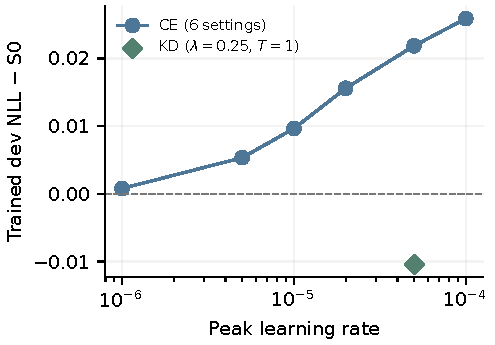
\includegraphics[width=\linewidth]{figures/partial_wt2_screen.pdf}
 \caption{Partial one-epoch WT2 screen from one student seed: six completed
 CE settings and the first completed KD setting. Values are trained dev
 NLL minus the common $S_0$ NLL. The remaining settings and full pilots are
 pending; this is not a final comparison or evidence for the new candidate.}
 \label{fig:partial}
\end{figure}

At the current checkpoint, all six trained CE screen endpoints are above
the $S_0$ dev NLL of 4.348015. Allowing step zero therefore selects $S_0$
for these screens. The first KD screen, with $\lambda=0.25$, $\tau=1$
and learning rate $5\times10^{-5}$, reaches 4.337590 after 294 updates.
Figure~\ref{fig:partial} shows exactly these completed settings. No full
candidate result or independent-seed variance is available yet.

The modern task uses a frozen no-think short-summary subset from
SmolTalk2. Complete response sequences must fit 512 tokens. The retained
66,946 examples are grouped by normalized source document, supplemented
by a fixed lexical near-duplicate screen. Preparation and continuation
contain 575,227 and 1,839,404 unique response targets, respectively.
Larger token budgets repeat examples and will be reported as such.
Tokenizer ID semantics, special tokens and actual encodings agree between
the pinned Qwen3 base models. Only assistant responses and their end
token are supervised; the dataset-specific summary instruction is retained.

The teacher will be adapted with LoRA and then frozen. The student will
use full-parameter training if the isolated GPU smoke permits it;
otherwise every student arm must use the same LoRA parameter set.
The continuation budget is determined by measured throughput before
adaptation endpoints. A CE pilot must establish development headroom,
with one preregistered earlier-$S_0$ fallback if necessary. No such modern
headroom or method result is available at this draft checkpoint.

Final modern reporting requires response NLL and fixed greedy ROUGE-L
against the synthetic reference responses. ROUGE does not establish
factual accuracy or general instruction capability. Development-selected
configurations will be frozen before test evaluation. Confirmatory
preparation seeds share pretrained base weights; a second teacher
adaptation seed is not an independent pretraining run.

\section{Cost, Limitations, and Pending Conclusions}
The program has a 230 GPU-hour ceiling, not a claim of consumed compute.
Accounting includes teacher adaptation, reference trajectories, extra
forwards, cache operations, search, discarded forks, evaluation and failed
attempts. Both student-update-matched and approximate total-GPU-hour
comparisons are required. Approximate cost controls must report the
achieved ratios. Reusing one CE cache across teachers can amortize its
cost, but the one-use reference cost must also be visible.

Implementation tests establish normalization, non-target ratios, gradient
equivalence, zero-KD equivalence, cache alignment, response masks and
chunked-gradient consistency. They do not establish model efficacy.
Shared-resource contention has already interrupted a disposable fork
smoke; incomplete attempts are retained as infrastructure records rather
than counted as method outcomes.

The completed study must distinguish teacher-specific information from
generic regularization, loss-scale effects and extra computation. If
current-student, mean-weight or identity-permuted controls match the
candidate, the corresponding independent-reference or teacher-structure
claim must be narrowed. Positive short-horizon utility cannot replace a
comparison with complete tuned CE and KD continuations. Failure to improve
generation metrics cannot be presented as improved task capability.

Historical results do not justify resurrecting a Grassmann-specific KD
advantage or a causal geometry claim. The old constant-positive diagnostic
has TP=15, FP=6, TN=0 and FN=0: its accuracy of 0.714286 is the majority
class fraction, balanced accuracy is 0.5, MCC is conventionally zero, and
continuous-score AUROC is 0.477778. These figures are not evidence of a
useful transfer predictor. The former modern continuation regime also
selected $S_0$ when allowed; it is kept separate from the new SFT study.

\section{Conclusion}
The implemented target correction is exactly adaptive CE/KD weighting at
temperature one. The pending empirical question is whether an independently
advancing CE reference supplies useful information beyond simpler sources
and coefficients at a defensible total cost. This draft does not answer
that question yet. Full pilots, informative controls, seed confirmation,
task evaluation and a final numerical audit are required before a
submission-ready conclusion can be written.

\bibliography{references}
\end{document}
